\documentclass[12pt,a4paper]{article}

% Encodage et langue
\usepackage[utf8]{inputenc}
\usepackage[T1]{fontenc}

% Packages mathématiques et typographiques
\usepackage{amsmath,amssymb}

% Packages requis par kableExtra (tableaux améliorés)
\usepackage{booktabs}
\usepackage{longtable}
\usepackage{array}
\usepackage{multirow}
\usepackage{xcolor}
\usepackage{colortbl}
\usepackage{float}

% Graphiques, mise en page, légendes
\usepackage{graphicx}
\usepackage{setspace}
\usepackage{geometry}
\geometry{margin=2.5cm}
\onehalfspacing
\usepackage{caption}

\title{Présentation des variables}
\author{José Manuel Rodríguez Caballero \\
	\small{STT-7335 Méthodes d'analyse de données}}
\date{\today}

\begin{document}
	\maketitle
	\tableofcontents
	
\section{Description du jeu de données}

Le présent rapport s’appuie sur un ensemble de 3443 vers, chacun annoté par un ensemble
de variables descriptives concernant l’auteur ou l’autrice, ainsi que par plusieurs
scores émotionnels.

\subsection{Détails des variables du jeu de données}
La liste ci-dessous décrit les colonnes du fichier source :

\begin{itemize}
	\item \textbf{poet\_id} : Identifiant unique associé à chaque poète.
	\item \textbf{poet} : Nom du poète ou de la poétesse.
	\item \textbf{suicidal} : Indicateur booléen précisant si l'auteur ou l'autrice
	s'est suicidé(e). Peut prendre la valeur \texttt{TRUE} ou \texttt{FALSE}.
	\item \textbf{period} : Période d'écriture (par exemple, \textit{Early} ou \textit{Modern}).
	\item \textbf{sex} : Sexe de la personne à l'origine du poème (\texttt{Male} ou \texttt{Female}).
	\item \textbf{heterosexual} : Indicateur booléen spécifiant l’orientation sexuelle,
	\texttt{TRUE} pour hétérosexuel(le), \texttt{FALSE} dans les autres cas.
	\item \textbf{date\_of\_birth} : Date de naissance de l'auteur ou de l'autrice.
	\item \textbf{date\_of\_death} : Date de décès de l'auteur ou de l'autrice, si disponible.
	\item \textbf{country\_of\_birth} : Pays de naissance de l'auteur ou de l'autrice.
	\item \textbf{poem\_title} : Titre du poème auquel le vers appartient.
	\item \textbf{n\_words} : Nombre de mots contenus dans le vers.
	\item \textbf{anger} : Score reflétant la présence de la colère dans le vers (valeur numérique).
	\item \textbf{anticipation} : Score reflétant l’anticipation (ou l'attente) véhiculée dans le vers
	(variable réponse principale de cette étude).
	\item \textbf{disgust} : Score reflétant la présence du dégoût dans le vers.
	\item \textbf{fear} : Score reflétant la présence de la peur dans le vers.
	\item \textbf{joy} : Score reflétant la présence de la joie dans le vers.
	\item \textbf{sadness} : Score reflétant la présence de la tristesse dans le vers.
	\item \textbf{surprise} : Score reflétant la présence de la surprise dans le vers.
	\item \textbf{trust} : Score reflétant la confiance véhiculée par le vers.
	\item \textbf{negative} : Score global regroupant des émotions à valence négative.
	\item \textbf{positive} : Score global regroupant des émotions à valence positive.
	\item \textbf{verse} : Position normalisée du vers dans le poème (\texttt{0} : début, \texttt{1} : fin).
\end{itemize}

Après nettoyage et vérification de la cohérence des données, le corpus final contient 3443
vers annotés. Le nombre de données manquantes est faible et n’impacte pas significativement
les analyses présentées ci-après.

\subsection{Provenance des données}
Les poèmes analysés dans cette étude ont été recueillis à partir de plusieurs sites Web,
dont les références figurent dans les données brutes. Chaque poème a été divisé en vers,
malgré un risque d’imperfection dans ce processus : un petit nombre de lignes
ne contiennent par exemple que des numéros ou des citations placées avant le début réel du poème.
Pour extraire les différentes composantes émotionnelles de chaque vers, nous avons
recouru à la bibliothèque \emph{syuzhet} du logiciel R. Celle-ci calcule divers scores
émotionnels (colère, joie, peur, etc.) et facilite ainsi l’analyse lexicale et sentimentale
des textes poétiques. Les dates de naissance, de décès et le pays de naissance des poètes
proviennent de Wikipédia. Enfin, la classification des poèmes selon la période de l'auteur
(début, milieu et fin) a été établie à l’aide de ChatGPT o1 pro.

\subsection{Orientation sexuelle}
Pour déterminer quels poètes sont hétérosexuels, nous avons utilisé le prompt suivant :

	\begin{verbatim}
	Génère un fichier CSV dont la première colonne s’intitule poet et la 
	deuxième colonne s’intitule heterosexual.  
	
	La colonne poet doit inclure les noms suivants :  
	- Adrienne Rich  
	- Alfred Edward Housman  
	- Anne Sexton  
	- Charlotte Mew  
	- Denise Levertov  
	- Edith Sitwell  
	- Edna St. Vincent Millay  
	- Hart Crane  
	- John Berryman  
	- John Davidson  
	- Lawrence Ferlinghetti  
	- Randall Jarrell  
	- Robert Lowell  
	- Sara Teasdale  
	- Sylvia Plath  
	- William Carlos Williams  
	
	La colonne heterosexual doit prendre la valeur 1 si le poète est 
	hétérosexuel, 0 s’il est homosexuel ou bisexuel, et NA si ces 
	informations ne sont pas clairement corroborées.  
	
	Merci de fournir simplement le tableau au format CSV, sans informations 
	superflues.
\end{verbatim}

Ce prompt a été appliqué à ChatGPT o1 pro.

\subsection{Données manquantes}
Parmi les 16 poètes étudiés, un seul n’a pas pu être classé selon son orientation sexuelle.
Nous projetons de récupérer cette donnée manquante en recourant à une analyse discriminante
linéaire, qui permettra de prédire l’orientation sexuelle en fonction des émotions
et d’autres variables.

\subsection{Objectif}
L’objectif de l’étude est d’évaluer dans quelle mesure les variables explicatives 
(par exemple, \textbf{anger}, \textbf{fear}, etc.) influencent la variable de réponse
\textbf{anticipation}.


\section{Présentation des variables}

\subsection{Statistiques descriptives}
Le tableau ci-dessous présente un résumé statistique (minimum, quartiles, médiane, moyenne, maximum)
des variables numériques, parmi lesquelles \textbf{anticipation}, \textbf{colère}, \textbf{peur}, etc.

\begin{table}
\centering
\caption{\label{tab:tab:summaryStatsFR}Variables numériques : statistiques récapitulatives (en français)}
\centering
\resizebox{\ifdim\width>\linewidth\linewidth\else\width\fi}{!}{
\begin{tabular}[t]{lrrrrrr}
\toprule
Variable & Min & 1er quartile & Médiane & Moyenne & 3e quartile & Max\\
\midrule
\cellcolor{gray!10}{Anticipation} & \cellcolor{gray!10}{0} & \cellcolor{gray!10}{0.00} & \cellcolor{gray!10}{0.0} & \cellcolor{gray!10}{0.15} & \cellcolor{gray!10}{0.00} & \cellcolor{gray!10}{3}\\
Colère & 0 & 0.00 & 0.0 & 0.11 & 0.00 & 4\\
\cellcolor{gray!10}{Confiance} & \cellcolor{gray!10}{0} & \cellcolor{gray!10}{0.00} & \cellcolor{gray!10}{0.0} & \cellcolor{gray!10}{0.13} & \cellcolor{gray!10}{0.00} & \cellcolor{gray!10}{3}\\
Dégoût & 0 & 0.00 & 0.0 & 0.12 & 0.00 & 2\\
\cellcolor{gray!10}{Joie} & \cellcolor{gray!10}{0} & \cellcolor{gray!10}{0.00} & \cellcolor{gray!10}{0.0} & \cellcolor{gray!10}{0.14} & \cellcolor{gray!10}{0.00} & \cellcolor{gray!10}{3}\\
\addlinespace
Nombre de mots & 1 & 5.00 & 7.0 & 6.76 & 8.00 & 40\\
\cellcolor{gray!10}{Négatif} & \cellcolor{gray!10}{0} & \cellcolor{gray!10}{0.00} & \cellcolor{gray!10}{0.0} & \cellcolor{gray!10}{0.33} & \cellcolor{gray!10}{1.00} & \cellcolor{gray!10}{4}\\
Peur & 0 & 0.00 & 0.0 & 0.17 & 0.00 & 4\\
\cellcolor{gray!10}{Positif} & \cellcolor{gray!10}{0} & \cellcolor{gray!10}{0.00} & \cellcolor{gray!10}{0.0} & \cellcolor{gray!10}{0.27} & \cellcolor{gray!10}{0.00} & \cellcolor{gray!10}{4}\\
Surprise & 0 & 0.00 & 0.0 & 0.08 & 0.00 & 2\\
\addlinespace
\cellcolor{gray!10}{Tristesse} & \cellcolor{gray!10}{0} & \cellcolor{gray!10}{0.00} & \cellcolor{gray!10}{0.0} & \cellcolor{gray!10}{0.19} & \cellcolor{gray!10}{0.00} & \cellcolor{gray!10}{3}\\
Vers & 0 & 0.24 & 0.5 & 0.49 & 0.74 & 1\\
\bottomrule
\end{tabular}}
\end{table}

\subsection{Distribution de la variable réponse}
La Figure~\ref{fig:hist_anticipation} illustre la distribution de la variable \textbf{anticipation}
sous forme d’histogramme. On constate une forte concentration des valeurs à 0 ainsi que
quelques occurrences plus élevées, bien que rares dans le corpus.

\begin{figure}[H]
	\centering
	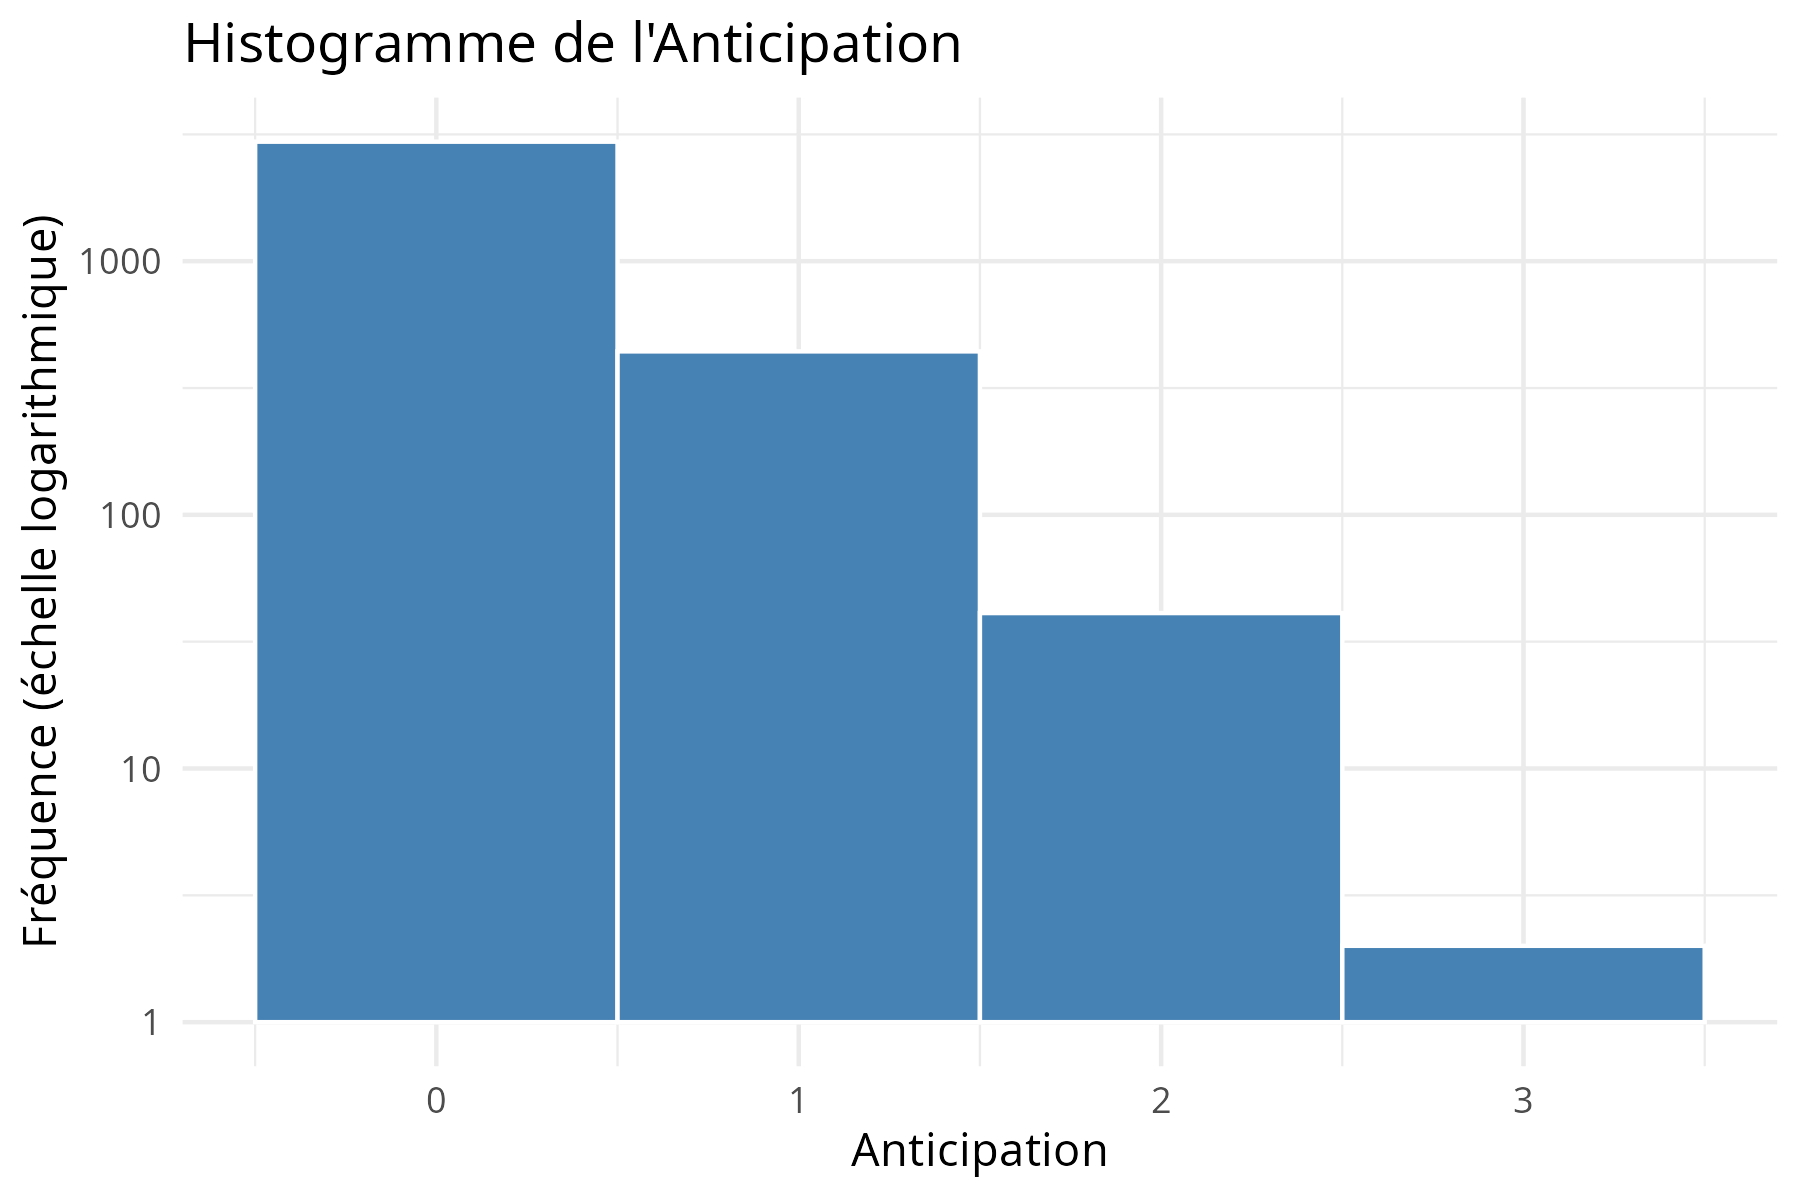
\includegraphics[width=1\textwidth]{figures/hist_anticipation.png}
	\caption{Histogramme de la variable \textbf{anticipation}.}
	\label{fig:hist_anticipation}
\end{figure}

\subsection{Distribution des variables explicatives}
La Figure~\ref{fig:hist_explicatives} présente des histogrammes pour chacune des variables
explicatives (émotions). L’échelle logarithmique sur l’axe des ordonnées facilite la visualisation
des queues de distribution et des valeurs rares.

\begin{figure}[H]
	\centering
	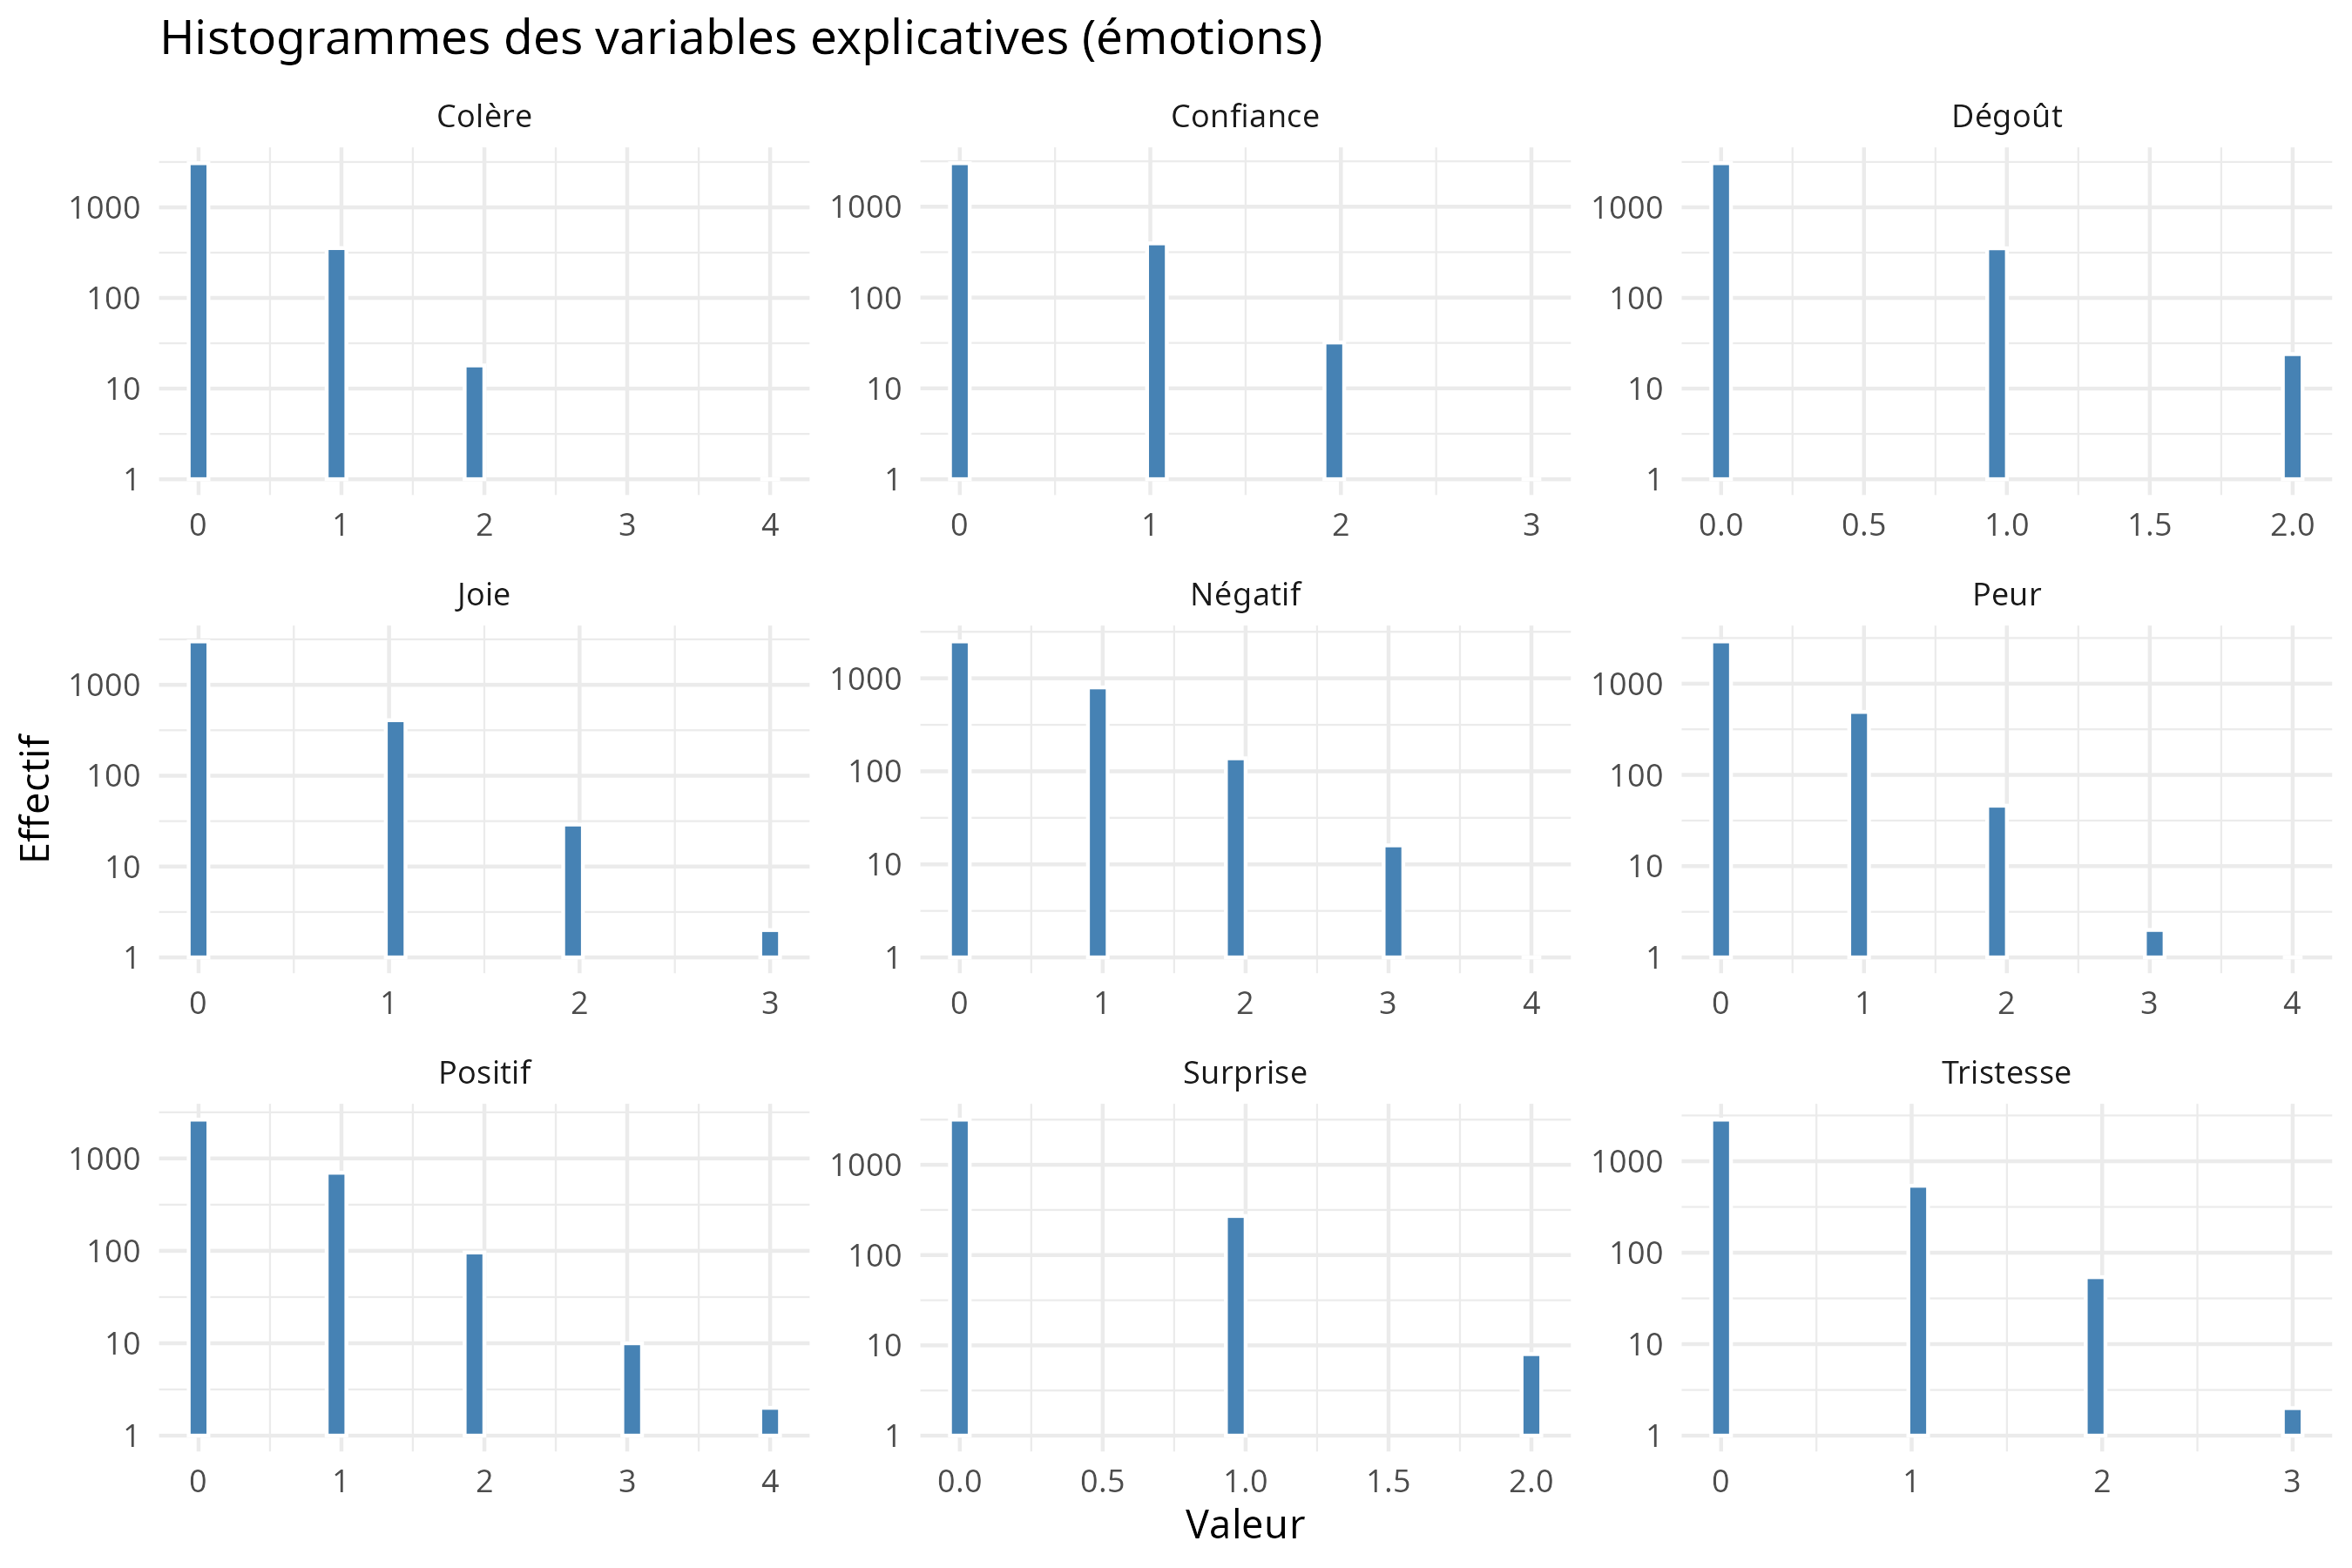
\includegraphics[width=1\textwidth]{figures/hist_all_explicatives.png}
	\caption{Histogrammes des variables explicatives (émotions), tracés en échelle logarithmique
		pour une meilleure lisibilité.}
	\label{fig:hist_explicatives}
\end{figure}

\subsection{Corrélations avec les autres variables émotionnelles}
La Figure~\ref{fig:cor_ggcorrplot} montre la matrice de corrélation entre \textbf{colère}, 
\textbf{anticipation}, \textbf{dégoût}, \textbf{peur}, \textbf{joie}, \textbf{tristesse}, 
\textbf{surprise}, \textbf{confiance}, \textbf{négatif} et \textbf{positif}. 
Ces corrélations ont été calculées selon la méthode de Kendall, puis réordonnées
par clustering hiérarchique pour mettre en évidence d’éventuels regroupements de variables.

\begin{figure}[H]
	\centering
	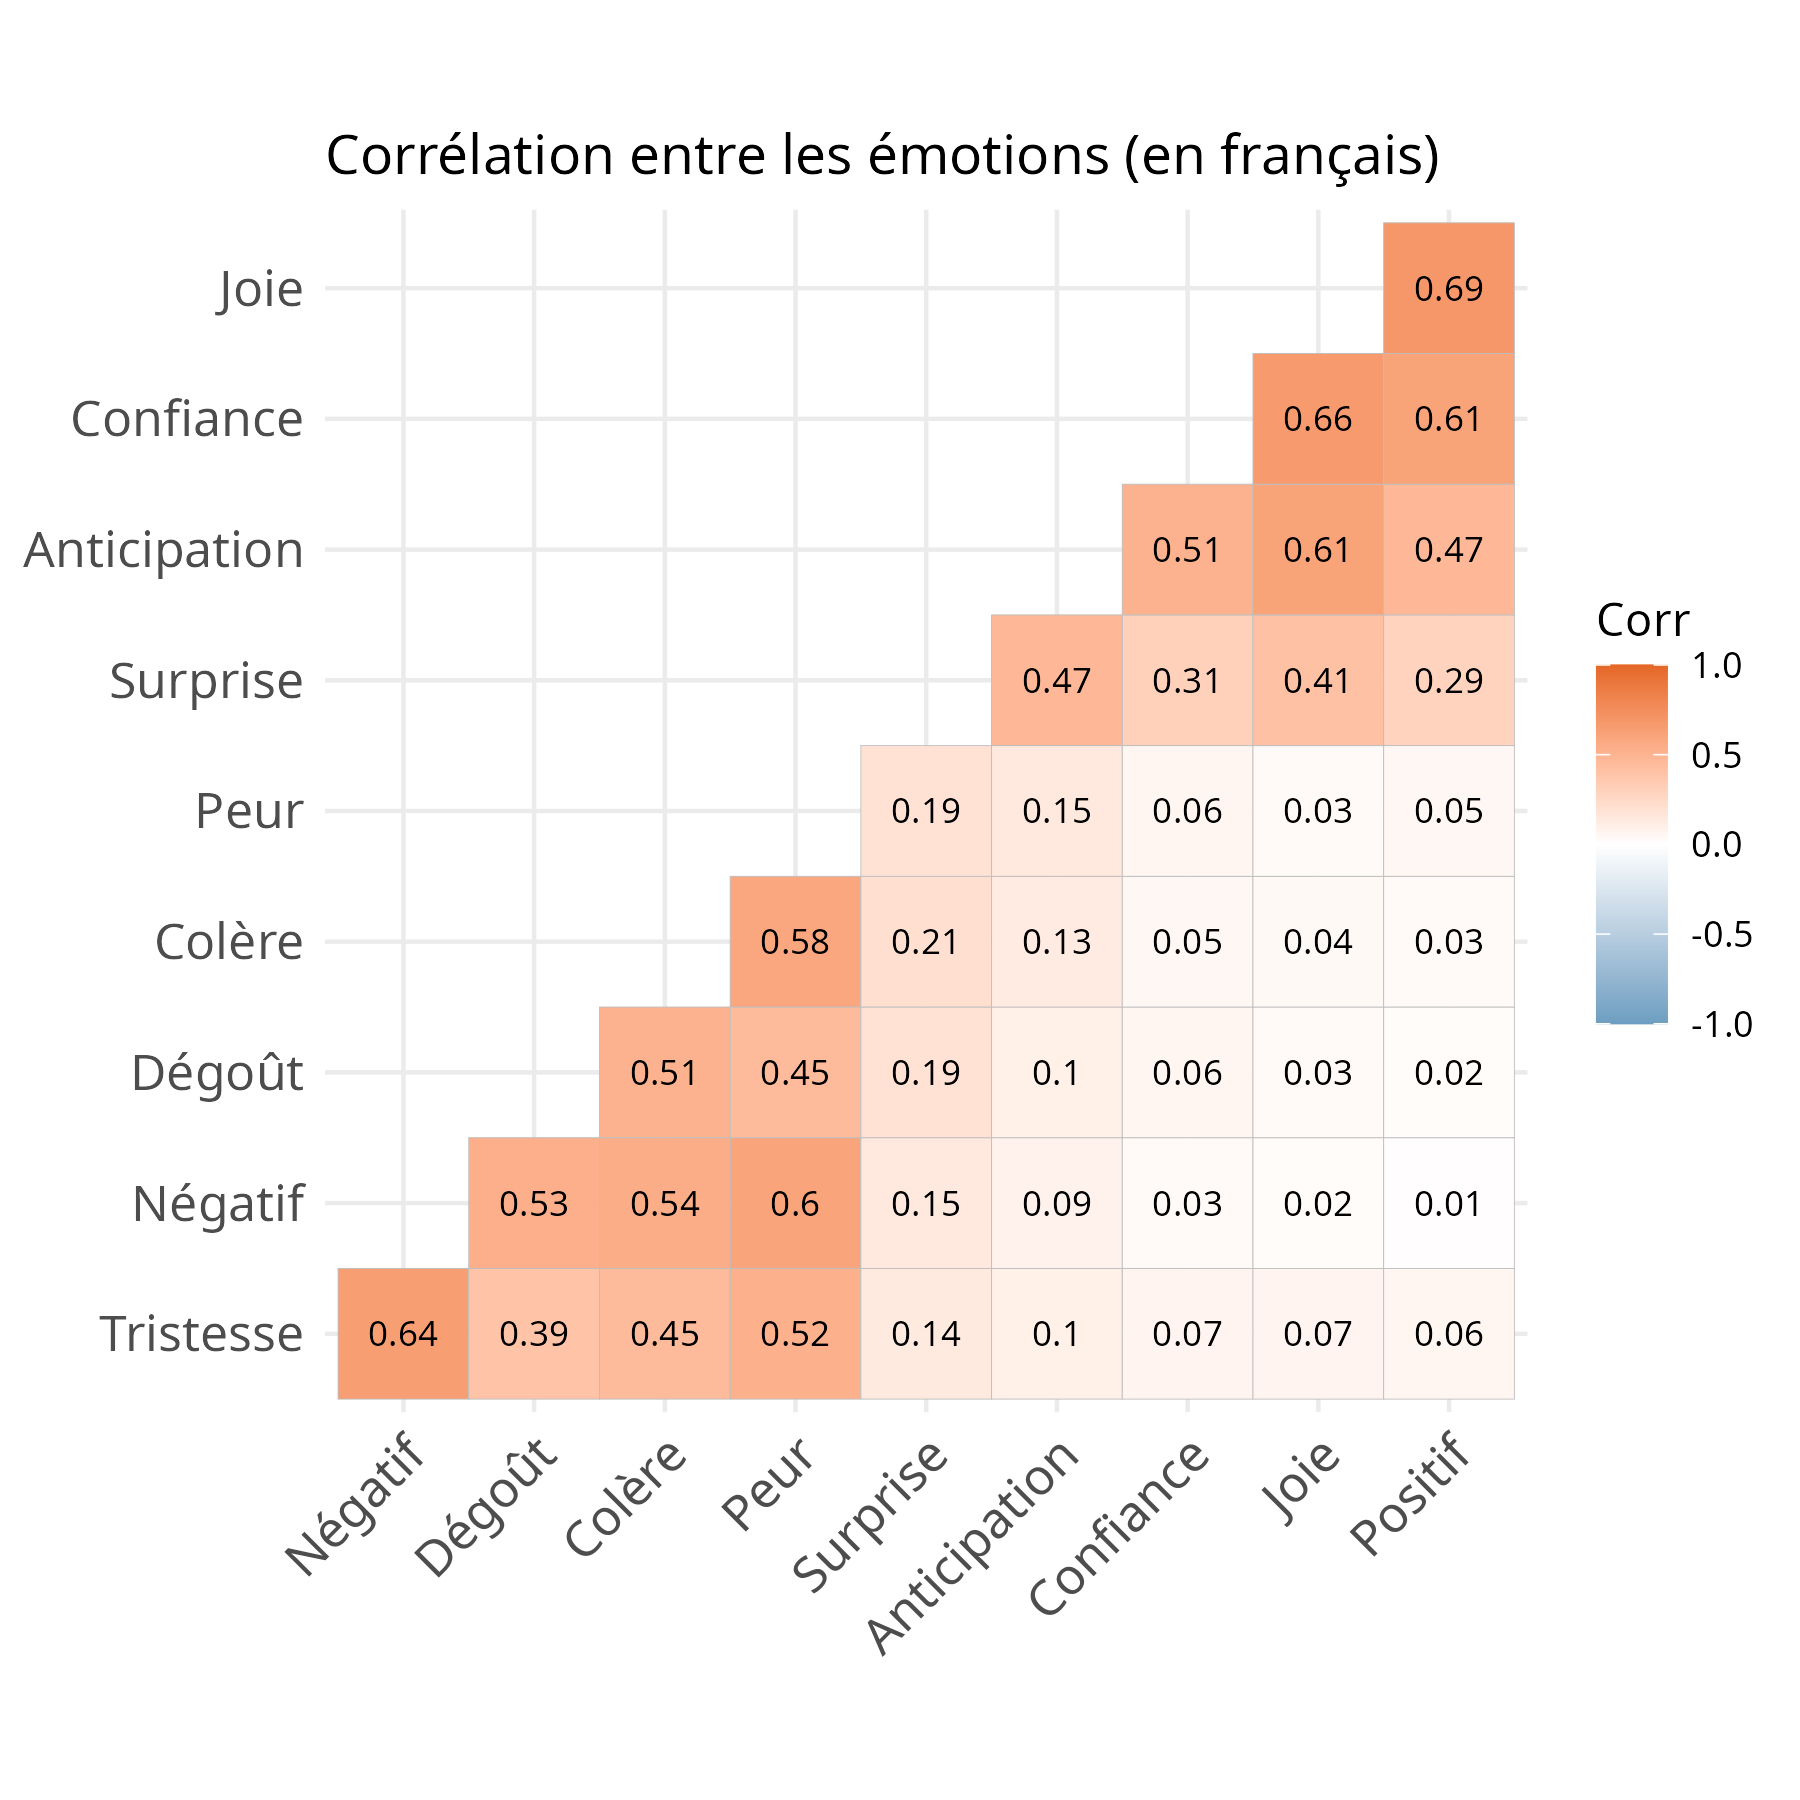
\includegraphics[width=1\textwidth]{figures/correlation_ggcorrplot.png}
	\caption{Matrice de corrélation (méthode : Kendall).}
	\label{fig:cor_ggcorrplot}
\end{figure}

\subsection{Fréquences d’anticipation = 0, 1, 2, 3 selon les variables catégorielles}
Les tableaux ci-dessous présentent la distribution des valeurs d’\textbf{anticipation}
(0, 1, 2, 3) en fonction de différentes variables catégorielles (\textbf{sexe},
\textbf{période}, \textbf{suicidal}, \textbf{heterosexual}).

\begin{table}[H]

\caption{Nombre de vers ayant Anticipation = 0,1,2,3 selon le Sexe.}
\centering
\begin{tabular}[t]{lrrrr}
\toprule
Sexe & Valeur\_0 & Valeur\_1 & Valeur\_2 & Valeur\_3\\
\midrule
Female & 1516 & 218 & 21 & 1\\
Male & 1443 & 223 & 20 & 1\\
\bottomrule
\end{tabular}
\end{table}
\begin{table}[H]

\caption{Nombre de vers ayant Anticipation = 0,1,2,3 selon la Période.}
\centering
\begin{tabular}[t]{lrrrr}
\toprule
Période & Valeur\_0 & Valeur\_1 & Valeur\_2 & Valeur\_3\\
\midrule
Early & 954 & 130 & 12 & 1\\
Later & 805 & 150 & 13 & 1\\
Middle & 1200 & 161 & 16 & 0\\
\bottomrule
\end{tabular}
\end{table}
\begin{table}[H]

\caption{Nombre de vers ayant Anticipation = 0,1,2,3 selon l'indicateur Suicidaire.}
\centering
\begin{tabular}[t]{lrrrr}
\toprule
Suicidaire & Valeur\_0 & Valeur\_1 & Valeur\_2 & Valeur\_3\\
\midrule
FALSE & 1618 & 194 & 11 & 0\\
TRUE & 1341 & 247 & 30 & 2\\
\bottomrule
\end{tabular}
\end{table}
\begin{table}[H]

\caption{Nombre de vers ayant Anticipation = 0,1,2,3 selon l'orientation sexuelle.}
\centering
\begin{tabular}[t]{lrrrr}
\toprule
heterosexual & Valeur\_0 & Valeur\_1 & Valeur\_2 & Valeur\_3\\
\midrule
FALSE & 871 & 136 & 16 & 0\\
TRUE & 1525 & 240 & 21 & 2\\
NA & 563 & 65 & 4 & 0\\
\bottomrule
\end{tabular}
\end{table}



\section{Analyse avec réduction de la dimension}
\subsection{Justification du choix et prétraitement}
Pour représenter plus clairement la structure multidimensionnelle des variables explicatives 
émotionnelles et faciliter leur interprétation, nous avons retenu 
l’\textit{analyse en composantes principales} (ACP). Celle-ci présente plusieurs intérêts :
\begin{itemize}
	\item \textbf{Réduction de la dimension :} En présence de nombreuses variables 
	potentiellement corrélées (par exemple \textbf{colère}, \textbf{peur}, 
	\textbf{dégoût}, etc.), l’ACP permet de synthétiser l’information sur quelques axes 
	principaux tout en conservant l’essentiel de la variance.
	\item \textbf{Visualisation :} Les deux ou trois premières composantes principales 
	offrent une représentation plus accessible, permettant de repérer des tendances 
	ou groupements dans l’espace des données.
	\item \textbf{Facilité d’interprétation :} Les poids (ou \textit{loadings}) associés 
	aux composantes principales mettent en évidence les variables qui contribuent 
	le plus à la variabilité globale, révélant souvent des oppositions claires 
	(émotions négatives vs. émotions positives, etc.).
\end{itemize}

Avant de procéder à l’ACP, \textbf{toutes les variables numériques ont été centrées et réduites} 
de manière à leur donner une échelle comparable. Ce prétraitement évite qu’une variable 
à variance élevée ne domine artificiellement les composantes.

\subsection{ACP et éboulis des valeurs propres}
La Figure~\ref{fig:pca_scree} présente l’éboulis (\textit{scree plot}) 
des valeurs propres de l’ACP, qui illustre la part de variance 
expliquée par chaque axe principal. On observe que les deux premiers axes 
expliquent environ \textbf{63,0\%} de la variance totale 
(\textbf{36,1\,\%} pour l’axe~1 et \textbf{26,9\,\%} pour l’axe~2), 
ce qui justifie l’utilisation d’un biplot bidimensionnel 
pour interpréter la majorité de l’information.

\begin{figure}[H]
	\centering
	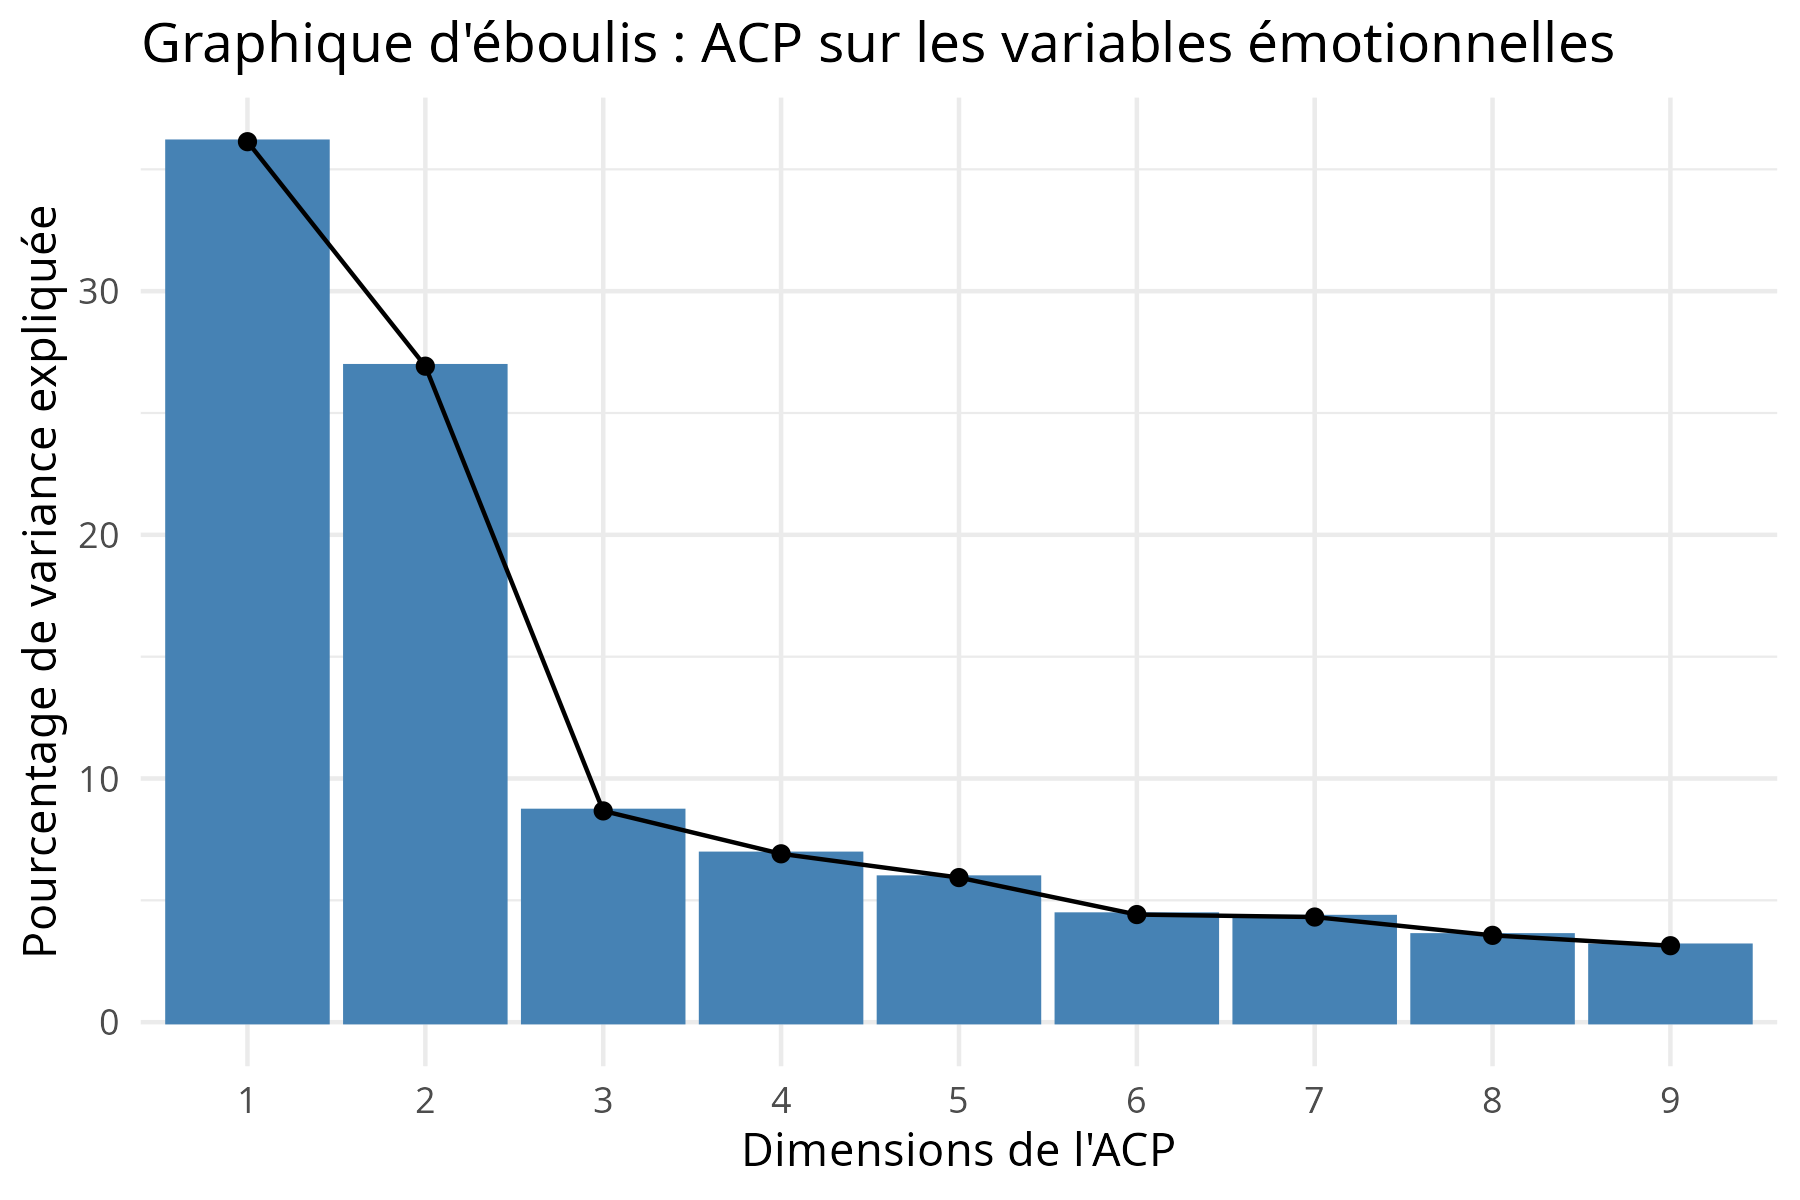
\includegraphics[width=0.65\textwidth]{figures_PCA/pca_screeplot.png}
	\caption{Éboulis (\textit{scree plot}) des composantes principales}
	\label{fig:pca_scree}
\end{figure}

\subsection{Biplot de l’ACP et interprétation}
La Figure~\ref{fig:pca_biplot} montre le \textit{biplot} des deux premières composantes, 
sur lequel les observations (chaque vers) sont projetées en points et 
les variables explicatives (émotions) en flèches. Pour faciliter la lecture, 
les points sont colorés en fonction de la valeur d’\textbf{anticipation}.

\begin{figure}[H]
	\centering
	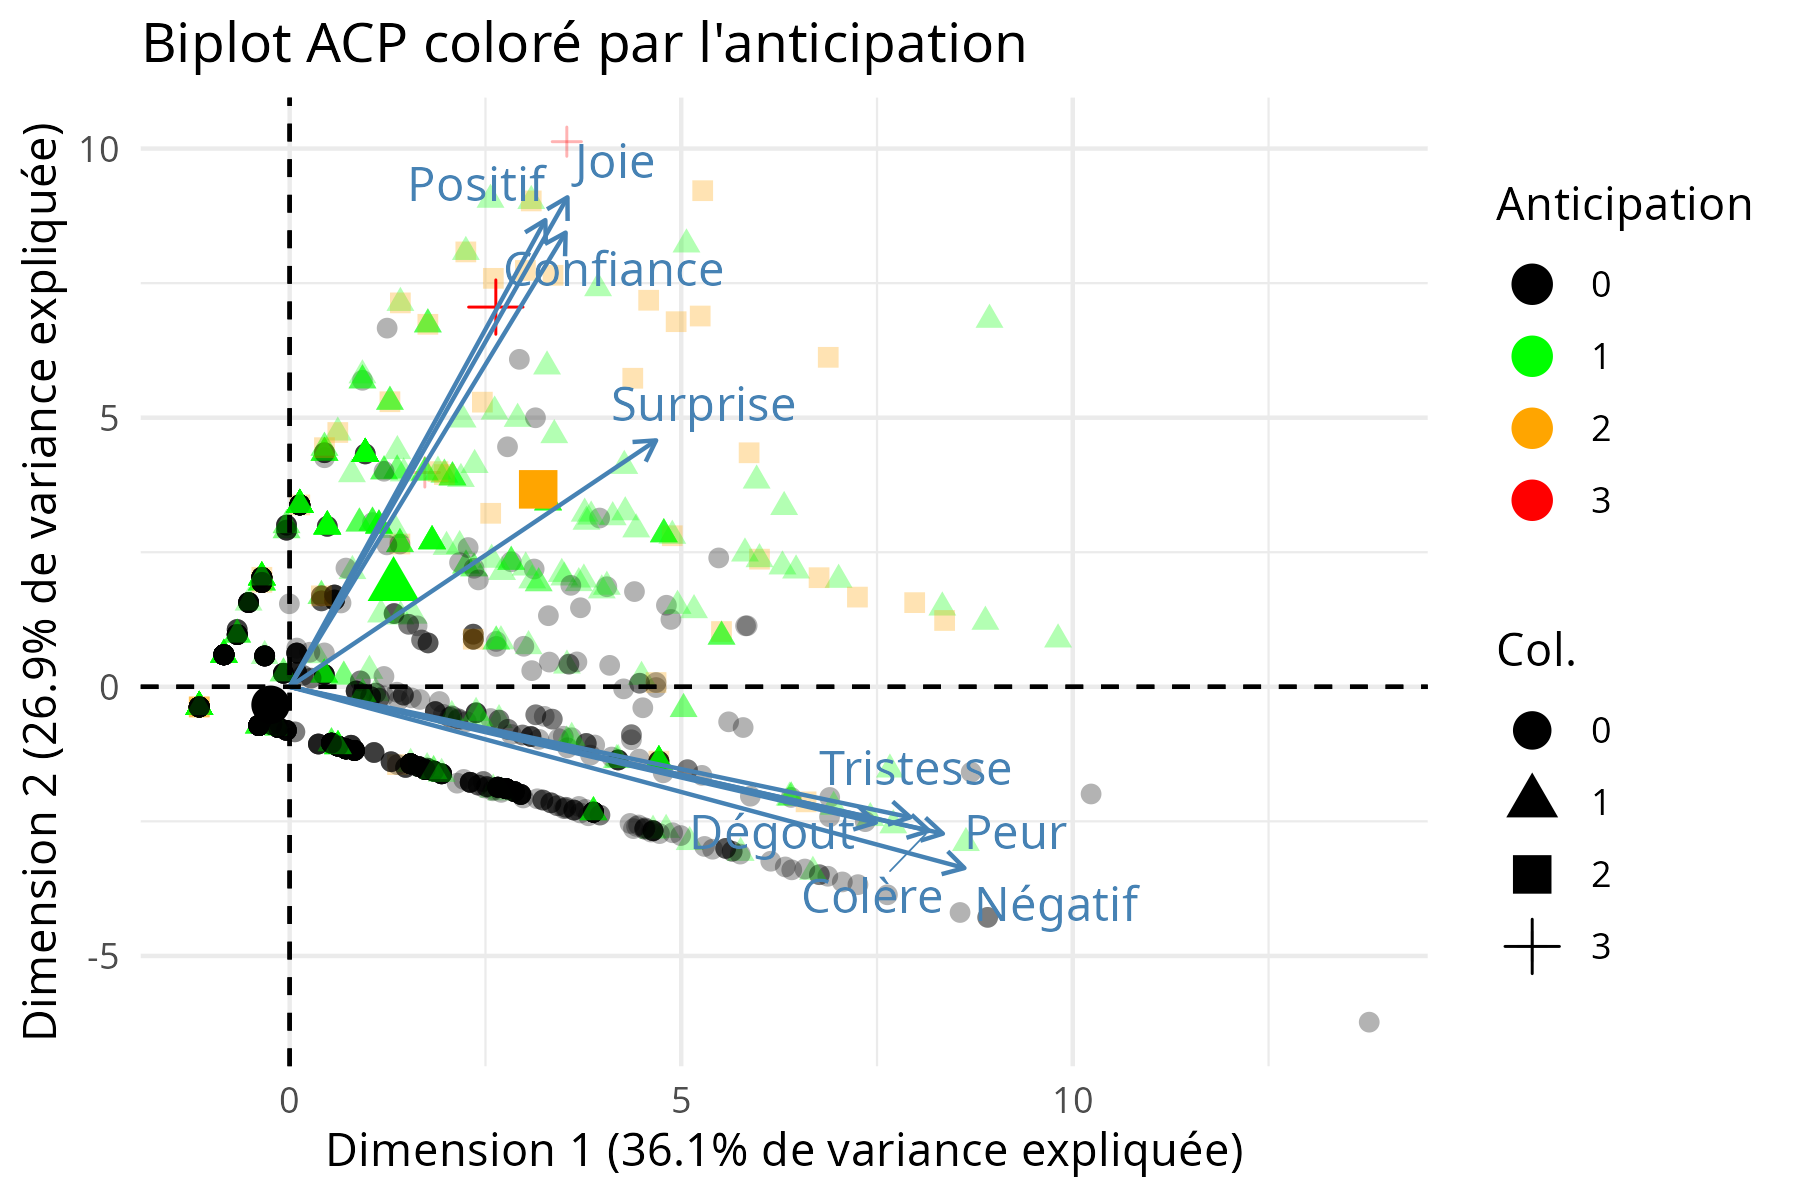
\includegraphics[width=0.75\textwidth]{figures_PCA/pca_biplot_anticipation.png}
	\caption{\textit{Biplot} de l’ACP, coloré selon la variable \textbf{anticipation}}
	\label{fig:pca_biplot}
\end{figure}

\paragraph{Interprétation des axes.}
\begin{itemize}
	\item \textbf{Axe 1 :} Il représente la croissance de l’expression des émotions, peu importe leur nature.
	\item \textbf{Axe 2 :} Il oppose les émotions positives aux émotions négatives.
\end{itemize}


\paragraph{Position de la variable \textbf{anticipation}.}
Sur le \textit{biplot}, \textbf{anticipation} grandit dans la direction positive de l’axe
associé aux émotions positives.


\subsection{Conclusion et perspectives}
\begin{itemize}
	\item L’ACP met en évidence \textbf{deux grands pôles émotionnels}, 
	opposant colère/peur/négatif à joie/confiance/positif, 
	avec un \textbf{rôle intermédiaire} pour \textbf{anticipation}.
	\item Les deux premiers axes expliquent la majeure partie de la variance 
	(environ \textbf{63,0\,\%}), ce qui facilite l’interprétation graphique et 
	justifie l’utilisation d’un biplot pour la visualisation.
	\item D’après cette analyse, la \textbf{valence émotionnelle} 
	(positif vs. négatif) représente la dimension la plus marquée dans nos données.
\end{itemize}

Pour aller plus loin, un modèle prédictif approfondi pourrait utiliser 
les composantes principales comme variables d’entrée afin de réduire 
le risque de \textit{surapprentissage} et faciliter l’interprétation. 
D’autres méthodes de réduction de dimension, telles que 
\texttt{t-SNE} ou \texttt{MDS}, mériteraient également d’être explorées 
pour repérer d’éventuelles structures non linéaires. 
Ainsi, la prochaine étape pourrait consister à comparer ces différentes approches 
avant de construire un modèle plus élaboré pour expliquer ou prédire 
\textbf{anticipation}.

	

	
\end{document}
